\documentclass[runningheads]{llncs}
\usepackage{graphicx}
\usepackage{amssymb,amsmath}
\usepackage{latexsym}
\usepackage{isabelle,isabellesym}

\newcommand{\equidom}[3]{{#1}\stackrel{#2}{\sim}{#3}}
\makeatletter
\newcommand{\superimpose}[2]
	{{\ooalign{$#1\@firstoftwo#2$\cr\hfil$#1\@secondoftwo#2$\hfil\cr}}}
\makeatother
\newcommand{\interf}{\leadsto}
\newcommand{\ninterf}{\mathrel{\mathpalette\superimpose{{\slash}{\leadsto}}}}

\begin{document}

\title{Formal Verification for A Buddy Allocation Model Specification}
%\title{Formal Verification for A Buddy Allocation Model Specification
%	\thanks{Supported by organization x.}}

\author{}
%\author{Ke Jiang\inst{1} \and
%		Yongwang Zhao\inst{2,3} \and
%		David San\'{a}n\inst{1} \and
%		Yang Liu\inst{1}}
%\authorrunning{Ke Jiang et al.}

\institute{}
%\institute{School of Computer Science and Engineering, \\
%			Nanyang Technological University, Singapore \\ 
%	\email{johnjiang,sanan,yangliu@ntu.edu.sg} \and
%			School of Computer Science and Engineering, \\
%			Beihang University, Beijing, China \and
%			Beijing Advanced Innovation Center for Big Data and Brain Computing, \\
%			Beihang University, Beijing, China \\
%	\email{zhaoyw@buaa.edu.cn}}

\maketitle


\begin{abstract}
Buddy allocation algorithms are widely adopted by memory management systems to manage the address space accessed by applications. However, errors in any stage of the development process of the memory management component, from the specification to the implementation, may lead to critical issues in other components using it. We apply formal methods to ensure the absence of any misbehavior. Rigorous mathematical proofs provide strong assurance to the development process. In this paper, we firstly present a specification for the buddy allocation algorithm. And thence we validate enough properties to guarantee functional correctness of this algorithm. Finally, we construct execution traces to verify the integrity for security. Through these efforts, we propose a buddy allocation model that provides both functional correctness and security. Also, we use interactive theorem prover Isabelle/HOL to carry out the verification work.

\keywords{Memory Specification \and
		Formal Verification \and
		Functional Correctness \and
		Security.}
\end{abstract}


\section{Introduction}
In the past several decades, buddy allocation algorithms have been applied in the memory management systems. Errors in any stage of the development process of the memory management component may lead to critical issues in other components who invoke it. To improve confidence on the reliability of the development process, verification of functional correctness and security properties is applied into each stage, from the specification level to the implementation level, even the machine code level. Formal methods have been successfully applied in the verification of many critical systems due to these methods provide strong assurance by rigorous mathematical proofs. Therefore, we apply formal methods to ensure the absence of any misbehavior during the development process of the buddy allocation model.

Many efforts have been put into the specification and verification of memory models. In the early cases, the memory model makes a set of operations available to programs and provides some guarantees on their behavior. These operations usually focus on reading and writing. The model built in~\cite{reg_higham} is such an example of formalizing memory models in terms of sequences of read and write events. Some of the later work even adds allocation and deallocation operations, but they are still abstract. 

In some models that only have read and write events, the property to verify is sequential consistency~\cite{reg_higham}, where model must behave as if it has received an ordered sequence of read and write operations. Promising non-existence of covert channels in memory model to guarantee isolation is another verifiable property as show in~\cite{reg_peter}. Paper~\cite{reg_rosu} proposes strong memory safety as the least restrictive formal definition of memory safety amenable for runtime verification.

The way in some work~\cite{reg_blazy,reg_mansky} of validating a memory model has several steps: firstly to build an axiomatic system that contains abstract operations and assumed properties; Secondly to give a specification of this model with semantics languages; Last to prove that the specification satisfy the axiomatic system.

In this paper, we propose a buddy allocation model, which supports both functional correctness and security. To achieve this goal, we develop a specification for buddy allocation algorithms by functional programming in Isabelle/HOL proof assistant. Our specification must consists of algorithm details as specific as possible for the sake of capturing any feature in the algorithms. Then we design a series of properties for functional correctness of the algorithm. After that, we apply theorem-proving method to prove these properties. To verify integrity for security, we construct execution traces based on event, and then prove that the operation of one domain on memory does not affect any other domains. So far, we have completed the construction and verification of the buddy allocation algorithm.

The following section briefly introduces the Isabelle/HOL verification environment. The next section is about the formalization of buddy allocation model including representation of our specification and proofs to properties for functional correctness. The verification of integrity for security is arranged in the following section. The last section is about the conclusions and future work.


\section{Isabelle/HOL Verification Environment}
Our specification and verification work is based on the interactive theorem prover Isabelle/HOL. HOL represents the Higher-Order Logical and Isabelle is its generic interactive theorem prover. In Isabelle/HOL, it is usual to employ functional programming method to define a function and to adopt theorem proving technique to reason a lemma or a theorem. For a gentle introduction to Isabelle/HOL see~\cite{reg_Isabelle/HOL}.

Apart from commonly used types like \emph{bool} and \emph{nat}, Isabelle offers notion \emph{datatype} to create a distinguished element to some existing types. Projection functions \emph{fst} and \emph{snd} comes with the tuple (\emph{$t_1$} $\times$ \emph{$t_2$}). Notions \emph{list} and \emph{set} are used as constructors to create a collection of same type. Operation \emph{cons} denoted by '$\#$' on a list means that adding an element to the head of list. The \emph{i}th component of a list \emph{xs} is written as \emph{xs}!\emph{i}. Notion \emph{THE} returns an arbitrary value unless the formula has a unique solution. Notion \emph{SOME} differs from \emph{THE} because it uses the
axiom of choice to pick any solution. Furthermore, $\lambda$-abstractions are also contained in terms like $\lambda$(\emph{x, y}). \emph{f x y}.

Non-recursive definition can be made with the \textbf{definition} command and the \textbf{primrec} function definition is used for primitive recursions. The notation {\isasymlbrakk} $A_1$;\dots;$A_n${\isasymrbrakk} $\Longrightarrow$ A represents an implication with assumptions $A_1$;\dots;$A_n$ and conclusion A. Isabelle mainly employs backward deduction, which means to prove the main goal, we must firstly prove subgoals which are decomposed from the main goal. It uses the rules of the reasoning like introduction, elimination, destruction rules, etc., as well as automatic provers such as \emph{SMT}.


\section{Formalization of Buddy Allocation Model}
The formalization of buddy allocation models consists of a specification for algorithms and proofs to properties for functional correctness. Generally, the buddy algorithms~\cite{reg_knowlton} in which each block is subdivided into two smaller blocks are the simplest and most common variety. The main idea is that when a larger block is split, it is divided into two smaller blocks, and each smaller block becomes a unique buddy to the other. A split block can only be merged with its unique buddy block, which then reforms the larger block they were split from. With this way, buddy memory system has little external fragmentation when compared with other dynamic allocation techniques.

In this paper, the difference is that we apply quartering way from Zephyr OS, an embedded system, for buddy allocation operations. This approach is more practical because it aims to pursue the efficiency. Since our specification requires a detailed description of the algorithms as well as the complex quartering way to describe, the foreseeable result is that it brings complexity to proofs than those abstract memory models. 

For functional correctness, we try to answer these questions which are the basic of later properties: Do the algorithms pick out the most suitable block from all the available blocks? Do the algorithms correctly adjust the type of the relevant memory blocks after allocation and deallocation? How do the algorithms make sure to execute the merging operation after deallocation? How does the specification ensure the correctness of the quad-tree structure? What invariants does the specification preserve? Do the algorithms satisfy some security properties? Answering these questions contributes to the construction of a reliability memory system.

\subsection{Memory Model Specification}
The specification begins with the structure of a quad-tree.
\begin{align*}
(set:\ 'a)\ tree = &Leaf\ (L:\ 'a)\ | \\
&Node\ (LL:\ 'a\ tree)\ (LR:\ 'a\ tree)\ (RL:\ 'a\ tree)\ (RR:\ 'a\ tree) \\
&for\ map: tree\_map
\end{align*}
The quad-tree constructed by induction contains two pieces of information: the memory block type (indicated as \emph{ALLOC} and \emph{FREE} respectively); a address tag occupied by a memory block (indicated as \emph{ID}). The mapping function \textbf{tree.set} assists to collect the leaves from a tree. With the help of the block \textbf{type} and the function \textbf{get\_level} in a quad-tree, allocated leaves or free leaves from different levels can be gathered by \textbf{allocsets}, \textbf{freesets} and \textbf{freesets\_level}. All used \emph{ID} labels are in \emph{idset}. To create a new leaf, we have to pick up a new \emph{ID} to this new leaf by the strategy of \emph{SOME p. p} $\notin$ \emph{idset}. Later, we will prove that with this strategy, all leaves have different \emph{ID} labels.

Based on the above structure of a quad-tree, next we specify two operations with the buddy algorithms: \textbf{alloc} and \textbf{free}. For \emph{rsize} (the size of requested memory block) in allocation operation, there is a function that maps it to the level of the quad-tree and returns the most suitable level \emph{rlv}. The concept of \emph{most suitable level} will be proved in the next subsection. For the specification, we only use levels for both memory blocks in the quad-trees and requested memory blocks. And the smaller the level, the larger size the memory block.

\begin{definition} [exists\_freelevel] \\
exists\_freelevel blo\_set lv $\equiv$ $\exists$l. l $\leq$ lv $\wedge$ $\exists$b $\in$ blo\_set. freesets\_level b l $\ne$ $\emptyset$
\end{definition}

\begin{definition} [freesets\_maxlevel] \\
freesets\_maxlevel blo\_set lv $\equiv$ \\
\phantom{x} \hspace{10pt} THE lmax. lmax $\leq$ lv $\wedge$ \\
\phantom{x} \hspace{60pt} $\exists$b $\in$ blo\_set. freesets\_level b lmax $\neq$ $\emptyset$ $\wedge$ \\
\phantom{x} \hspace{60pt} $\forall$l $\leq$ lv. $\exists$b $\in$ blo\_set. freesets\_level b l $\ne$ $\emptyset$ $\longrightarrow$ l $\leq$ lmax
\end{definition}

\begin{definition} [Allocation Operation] \\
alloc blo\_set rlv $\equiv$ \\
\phantom{x} \hspace{10pt} if exists\_freelevel blo\_set rlv then \\
\phantom{x} \hspace{20pt} lmax = freesets\_maxlevel blo\_set rlv \\
\phantom{x} \hspace{20pt} if lmax = rlv then \\
\phantom{x} \hspace{30pt} btree = SOME b. b $\in$ blo\_set $\wedge$ freesets\_level b rlv $\ne$ $\emptyset$ \\
\phantom{x} \hspace{30pt} l = SOME l. l $\in$ freesets\_level btree rlv \\
\phantom{x} \hspace{20pt} else \\
\phantom{x} \hspace{30pt} btree = SOME b. b $\in$ blo\_set $\wedge$ freesets\_level b lmax $\ne$ $\emptyset$ \\
\phantom{x} \hspace{30pt} l = split (SOME l. l $\in$ freesets\_level btree lmax) (rlv - lmax) \\
\phantom{x} \hspace{10pt} else False
\end{definition}

The first step of allocation is to check whether there is a quad-tree in \emph{blo\_set} (the memory pool tree collection), that has such free memory blocks whose level is less than or equal to \emph{rlv}. This step is done by \textbf{exists\_freelevel}, and if it returns \emph{False} then the allocation progress stops. Otherwise, the next step conducted by \textbf{freesets\_maxlevel} is to return the maximum level among all levels with free memory blocks. If the maximum level is equal to \emph{rlv}, then any free memory block in \emph{rlv} is to be allocated. If not, any free memory block in the maximum level is to be conducted by \textbf{split} showed in Fig. \ref{fig1} until free memory block in \emph{rlv} appears and then be allocated. The type of the assigned leaf is set to \emph{ALLOC}.

\begin{figure}
\centering
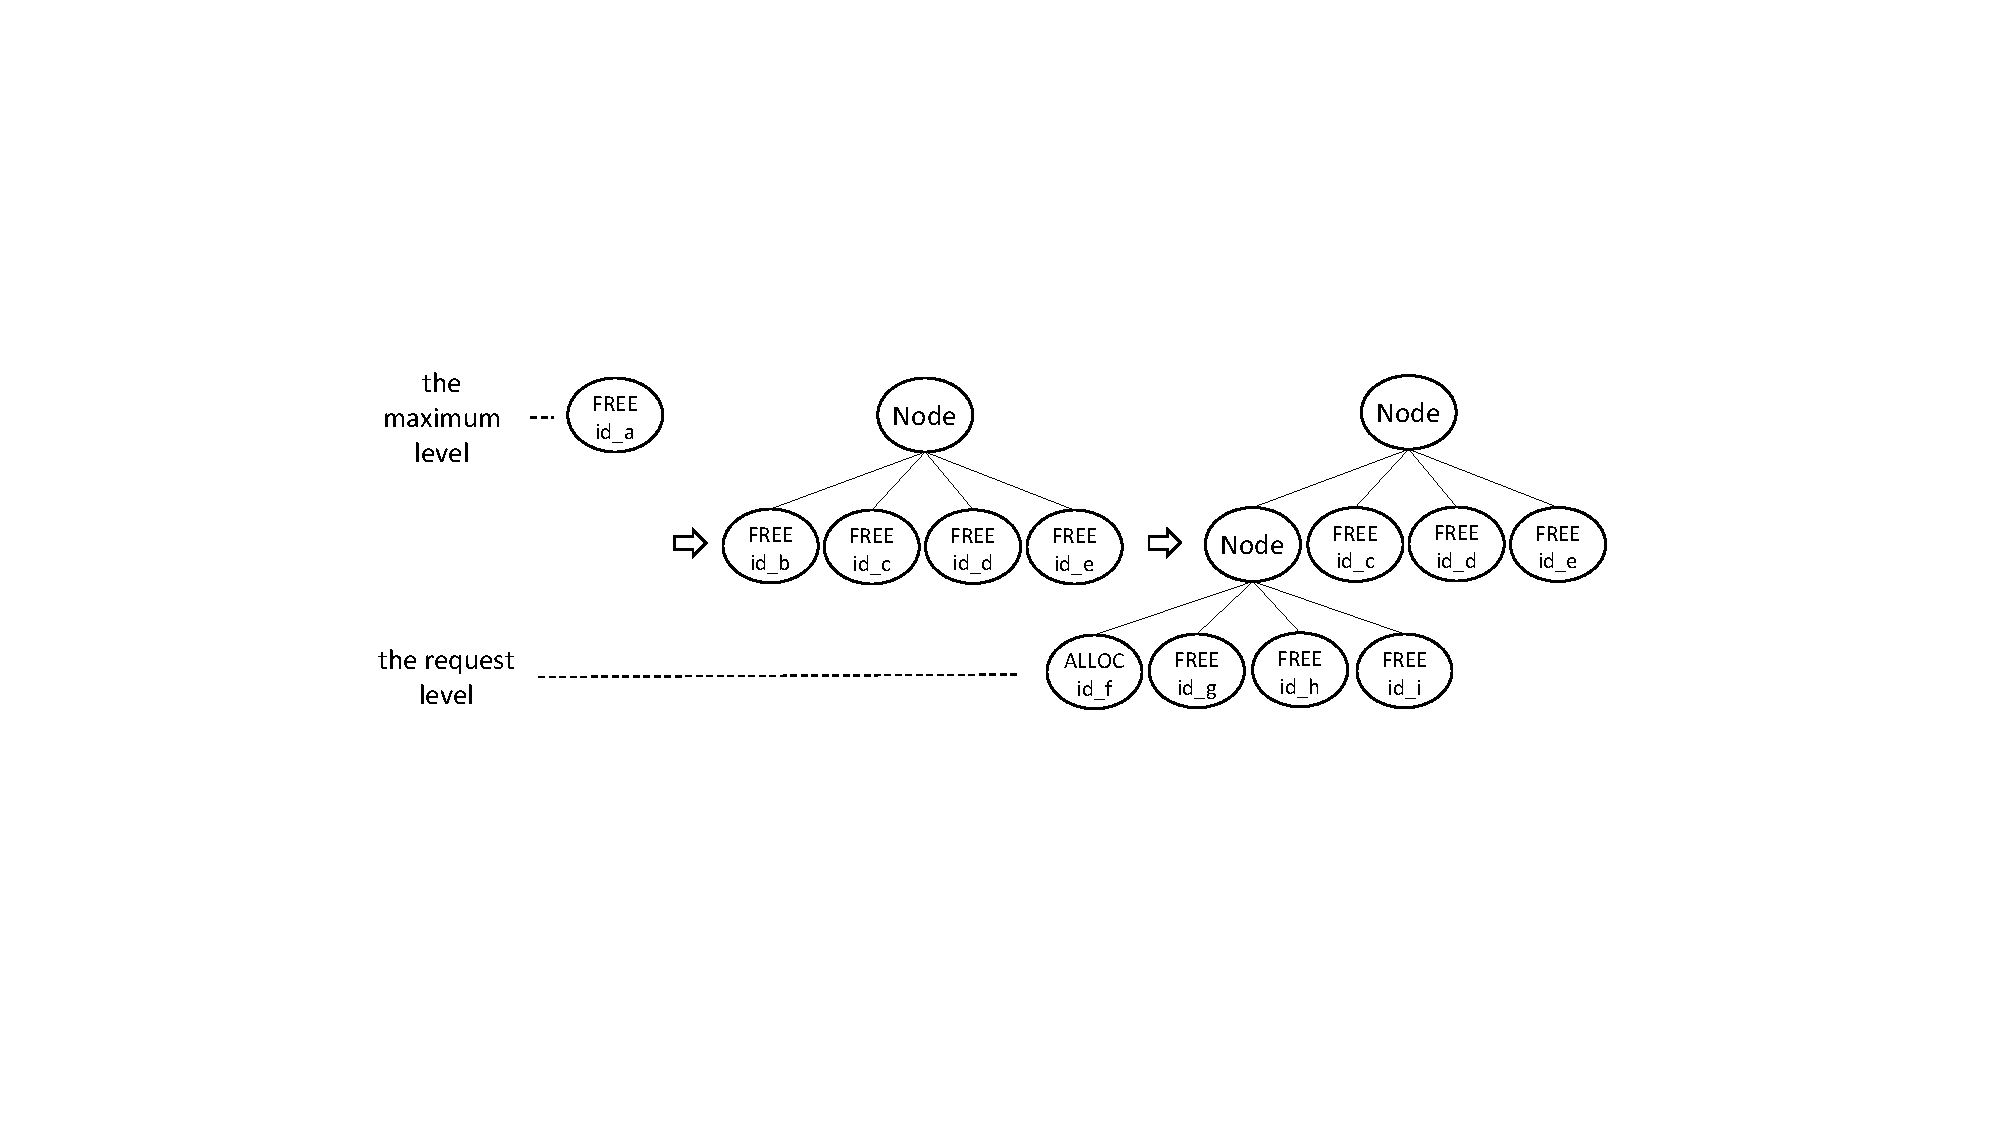
\includegraphics[width=1\textwidth]{fig1.pdf}
\caption{The progress of dividing a free memory block}
\label{fig1}
\end{figure}

\begin{definition} [Deallocation Operation] \\
free blo\_set b $\equiv$ \\
\phantom{x} \hspace{10pt} if $\exists$btree $\in$ blo\_set. b $\in$ tree.set btree then \\
\phantom{x} \hspace{20pt} if type b = FREE then False \\
\phantom{x} \hspace{20pt} else btree = THE t. t $\in$ blo\_set $\wedge$ b $\in$ tree.set t \\
\phantom{x} \hspace{40pt} merge (reset btree b FREE) \\
\phantom{x} \hspace{10pt} else False
\end{definition}

The deallocation progress firstly checks whether there is a quad-tree in \emph{blo\_set} that the occupied memory block to be released belongs to this tree. If there is no such tree, the procedure returns \emph{False}. Next, if the type of the occupied memory block is \emph{FREE}, the progress also returns \emph{False}. When all conditions are met, the memory block is returned to the tree it belongs to, thereafter merging operation is executed. The merging operation is to combine all free memory blocks that belong to the same parent tree showed in Fig. \ref{fig2}.

\begin{figure}
\centering
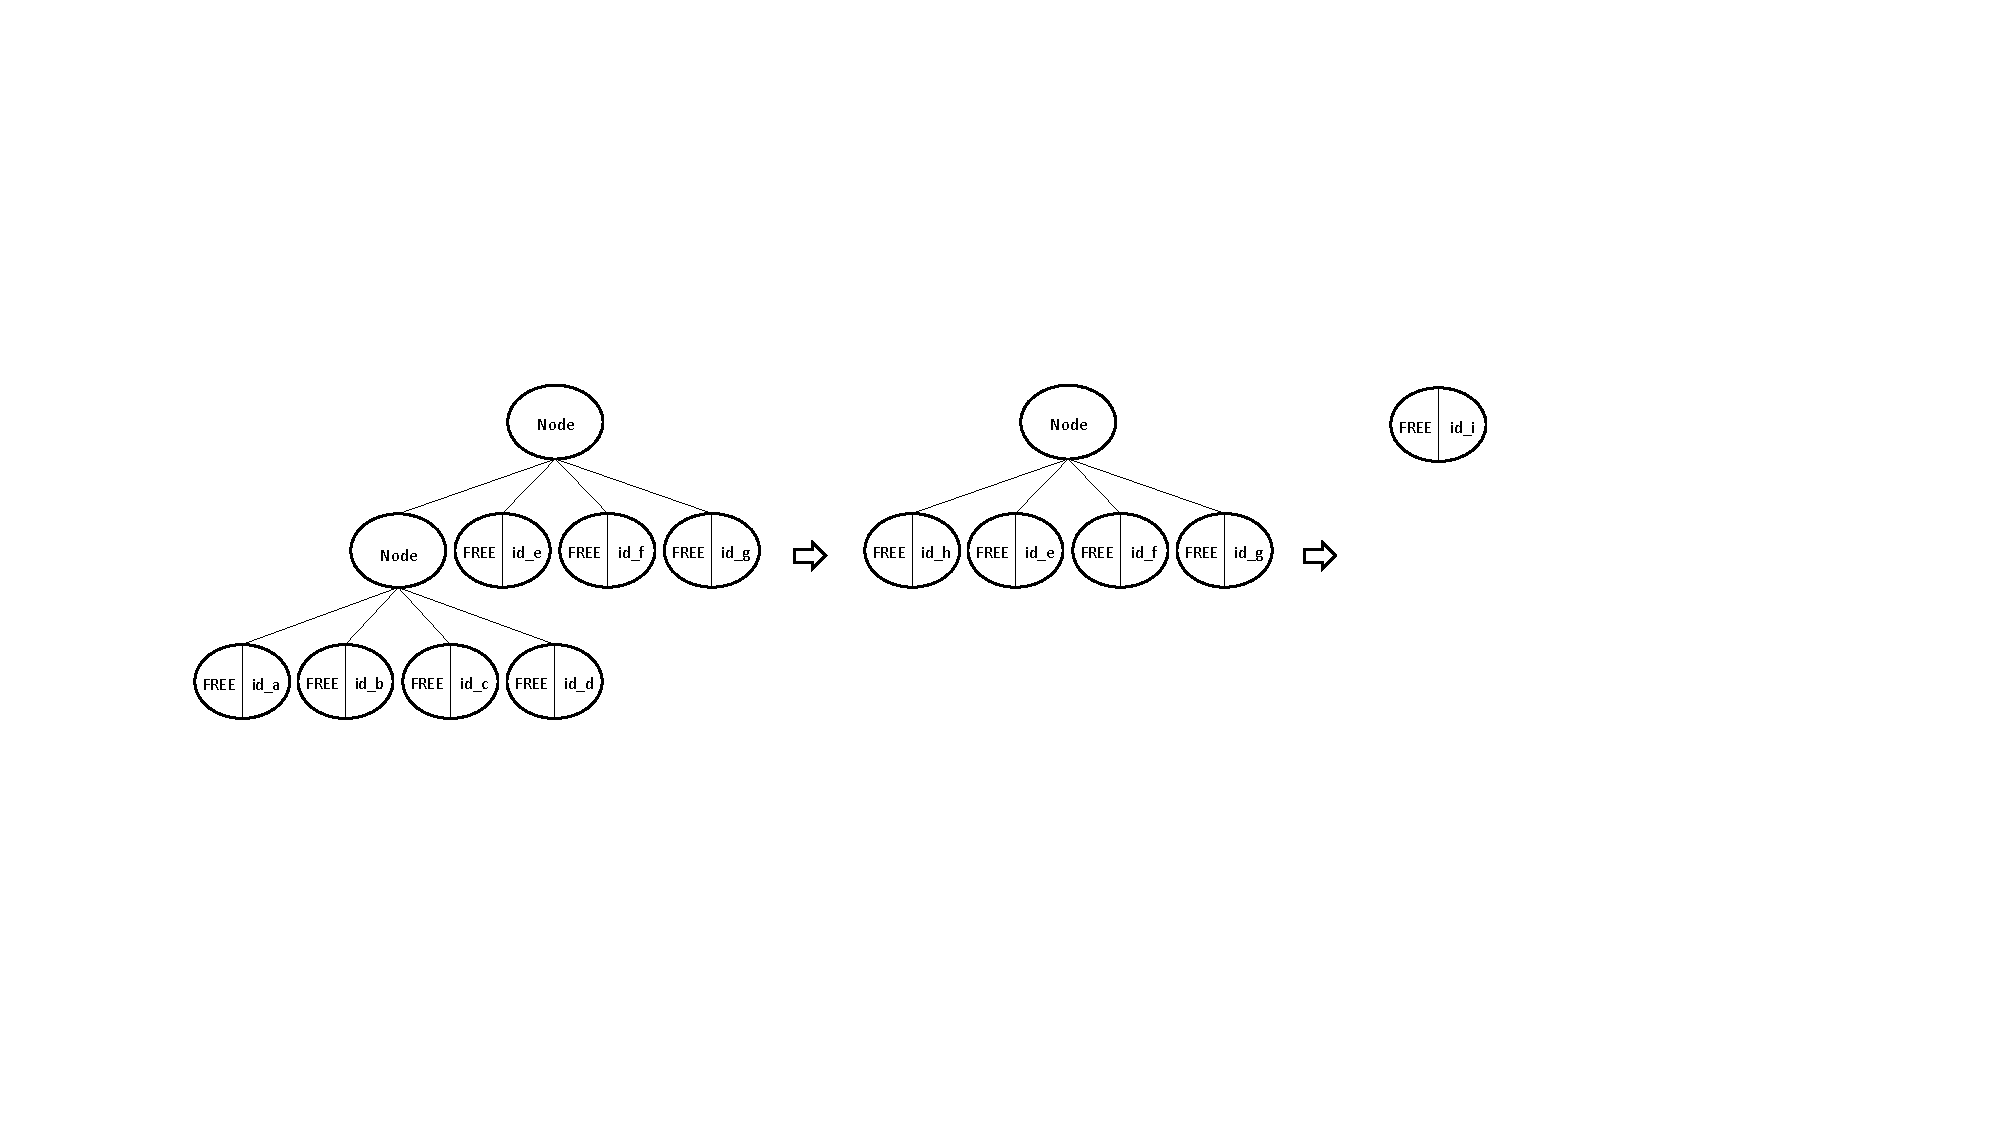
\includegraphics[width=1\textwidth]{fig2.pdf}
\caption{The progress of merging all free memory blocks}
\label{fig2}
\end{figure}

Owing to space constraints, the \emph{split} and the \emph{merge} operations constructed by induction are not described in detail. At this point, we have done the specification for the buddy memory algorithms. Next, we are going to verify the properties to guarantee the functional correctness of this specification.


\subsection{Memory Model Properties}
Once the specification is finished, the preconditions $\&$ postconditions for functions as well as the invariants are to be raised up to ensure the functional correctness of the specification. We give preconditions and postconditions in the first place.

\begin{definition} [Allocation Failure] \\
$\neg$ exists\_freelevel blo\_set rlv $\longrightarrow$ fst (alloc blo\_set rlv) = blo\_set
\label{pp1}
\end{definition}

\begin{definition} [Freesets for Direct Allocation] \\
exists\_freelevel blo\_set rlv $\wedge$ freesets\_maxlevel blo\_set rlv = rlv $\longrightarrow$ \\
\phantom{x} \hspace{10pt} $\exists$l. l $\in$ freesets blo\_set $\wedge$ l $\notin$ freesets fst (alloc blo\_set rlv) $\wedge$ \\
\phantom{x} \hspace{10pt} freesets blo\_set = freesets fst (alloc blo\_set rlv) $\cup$ $\lbrace$l$\rbrace$
\label{pp2}
\end{definition}

\begin{definition} [Allocsets for Direct Allocation] \\
exists\_freelevel blo\_set rlv $\wedge$ freesets\_maxlevel blo\_set rlv = rlv $\longrightarrow$ \\
\phantom{x} \hspace{10pt} $\exists$l. l $\notin$ allocsets blo\_set $\wedge$ l $\in$ allocsets fst (alloc blo\_set rlv) $\wedge$ \\
\phantom{x} \hspace{10pt} allocsets fst (alloc blo\_set rlv) = allocsets blo\_set $\cup$ $\lbrace$l$\rbrace$
\label{pp3}
\end{definition}

\begin{definition} [Allocsets for Indirect Allocation] \\
exists\_freelevel blo\_set rlv $\wedge$ freesets\_maxlevel blo\_set rlv $\neq$ rlv $\longrightarrow$ \\
\phantom{x} \hspace{10pt} $\exists$l. l $\notin$ allocsets blo\_set $\wedge$ l $\in$ allocsets fst (alloc blo\_set rlv) $\wedge$ \\
\phantom{x} \hspace{10pt} allocsets fst (alloc blo\_set rlv) = allocsets blo\_set $\cup$ $\lbrace$l$\rbrace$
\label{pp4}
\end{definition}

\begin{definition} [Deallocation failure 1] \\
$\nexists$btree $\in$ blo\_set. b $\in$ tree.set btree $\longrightarrow$ fst (free blo\_set b) = blo\_set
\label{pp5}
\end{definition}

\begin{definition} [Deallocation failure 2] \\
$\exists$btree $\in$ blo\_set. b $\in$ tree.set btree $\wedge$ type b = FREE $\longrightarrow$ \\
\phantom{x} \hspace{10pt} fst (free blo\_set b) = blo\_set
\label{pp6}
\end{definition}

\begin{definition} [Allocsets for Deallocation Success] \\
$\exists$btree $\in$ blo\_set. b $\in$ tree.set btree $\wedge$ type b $\neq$ FREE $\longrightarrow$ \\
\phantom{x} \hspace{10pt} allocsets blo\_set = allocsets fst (free blo\_set b) $\cup$ $\lbrace$b$\rbrace$
\label{pp7}
\end{definition}

As the names suggest, Def. \ref{pp1} gives such an implication: if there is not a quad-tree in \emph{blo\_set} that has free memory blocks whose level is less than or equal to \emph{rlv}, nothing is to be changed because of the allocation failure. Def. \ref{pp2} and Def. \ref{pp3} respectively describe the block to be allocated no longer belongs to the free sets and is part of allocated sets during the direct allocation process. Def. \ref{pp4} says that a new block created from splitting a bigger block is allocated and belongs to the allocated sets during indirect allocation, which means \emph{split} operation is needed. The next two Def. \ref{pp5} and Def. \ref{pp6} guarantee nothing to be changed during the deallocation process because of the non-existence of such a quad-tree that the block to be released belongs to or the type of the block to be freed is \emph{FREE}. The last Def. \ref{pp7} tells that the block to be deallocated does not belong to allocated sets any more.

\begin{theorem}
The buddy allocation specification satisfies all the preconditions and postconditions above.
\end{theorem}

\begin{proof}
All parts can be formally proved by induction on the type of a quad-tree, including leaf and node types. And the proofs on node type can be conducted by another induction which is on the height of the derivation.
\end{proof}

Through preconditions and postconditions, the specification can be proved that it partly follows the expectations of the algorithms. Next to guarantee that the algorithms pock out the most suitable block, two properties have to be proved: 1. the correctness of the mapping from the request memory block size to the level of the quad-tree. 2. the correctness of the quad-tree hierarchical  structure. Here are these two properties.

\begin{definition} [Mapping Request Sizes to Allocation Levels] \\
output\_level blo\_list rsize $\equiv$ THE l. l $<$ L blo\_list $\wedge$ rsize $\le$ blo\_list ! l $\wedge$ \\
\phantom{x} \hspace{10pt} (L blo\_list $>$ 1 $\wedge$ l $<$ L blo\_list - 1) $\longrightarrow$ rsize $>$ L blo\_list ! (l+1)
\end{definition}

Static linked list \emph{blo\_list} is used to store the size of block for each level in a quad-tree. For example, the size of root is 1024\emph{M} and the first level is 256\emph{M}, then \emph{blo\_list}!0 is equal to 1024 and \emph{blo\_list}!1 is 256. The \emph{blo\_list} is a strictly decreasing list. Function \textbf{L} is used to get the length of a list. As mentioned above, the smaller the level, the larger size the memory block. The most suitable block means that its size has to be greater than or equal to the size of request block, and there is no smaller block that meets this condition. Through this definition, the most suitable block is picked up from \emph{blo\_list}, and then mapped to the correct level of the quad-tree by the index of \emph{blo\_list}. Some lemmas ensure the correctness of this definition.

\begin{lemma}
L blo\_list $>$ 0 $\wedge$ rsize $\leq$ blo\_list ! (L blo\_list - 1) $\longrightarrow$ output\_level blo\_list rsize = L blo\_list - 1
\end{lemma}

\begin{lemma}
L blo\_list $>$ 1 $\wedge$ l $<$ L blo\_list - 1 $\wedge$ rsize $\leq$ blo\_list ! l $\wedge$ rsize $>$ blo\_list ! (l + 1) $\longrightarrow$ output\_level blo\_list rsize = l
\end{lemma}

\begin{proof}
By unfolding the definition of output\_level, two aspects including existence and uniqueness have to be proved for the notion THE. The first part existence can be proved by the given assumptions. The remaining part uniqueness can be proved by the strictly decreasing blo\_list.
\end{proof}

Next, we introduce a lemma alone to prove the correctness of a quad-tree structure from the aspect of its levels. The \textbf{root} checks whether the tree is a root tree and \textbf{child} gives us all immediate child nodes.

\begin{lemma}
(root btree $\longrightarrow$ get\_level btree = 0) $\wedge$ (get\_level btree = l $\wedge$ l $\geq$ 0 $\wedge$ chtree $\in$ child btree $\longrightarrow$ get\_level chtree = l + 1)
\end{lemma}

\begin{proof}
This lemma can be formally proved by induction on the height of the derivation.
\end{proof}

Until now, we have already proved the correctness of the mapping operation and the hierarchical structure of a quad-tree. Then we can deduce the following theorem to guarantee the property of picking out the most suitable memory block.

\begin{theorem}
The buddy allocation specification picks out the most suitable memory block and operates on the correct level in a quad-tree.
\end{theorem}

The algorithms are designed to avoid the fragmentation by merging operation which is invoked in the process of deallocation. Whether this operation is executed correctly can not be proved from the surface. In order to prove this property, we still start from the structural correctness of the quad-tree. Considering the fact that there is not such a node whose four child nodes are all leaves and their types are \emph{FREE} after merging operation, a definition to check whether a tree is like this can be constructed as follows. The \textbf{leaf} is to check whether the tree is a leaf.

\begin{definition} [Four Free Leaves Belong to The Same Node] \\
is\_FFL btree $\equiv$ $\forall$chtree $\in$ child btree. leaf chtree $\wedge$ type chtree = FREE
\end{definition}

Fig. \ref{fig2} can explain this definition well. Just like the subtree in the lower left corner of the first picture, four child nodes are all leaves and their types are \emph{FREE}. Therefore, merging operation is necessary during the progress of deallocation to handle this situation. The following are the lemmas that ensure the non-existence of such \emph{FFL} trees after allocation and deallocation operations if non-existence of such trees in preconditions.

\begin{lemma}
$\forall$b $\in$ blo\_set. $\neg$ is\_FFL b $\longrightarrow$ $\forall$b $\in$ fst (alloc blo\_set rlv). $\neg$ is\_FFL b
\end{lemma}

\begin{lemma}
$\forall$b $\in$ blo\_set. $\neg$ is\_FFL b $\longrightarrow$ $\forall$b $\in$ fst (free blo\_set b). $\neg$ is\_FFL b
\end{lemma}

\begin{proof}
Apply cases to these two lemmas after folding the definitions of allocation and deallocation operations. For each cases, they can be proved by induction on the height of the derivation.
\end{proof}

After memory initialization, assuming that all blocks to be allocated are the original ones which are not split, this beginning of the moment satisfies non-existence of \emph{FFL} trees among all quad-trees because all available blocks are seen as root trees. This assertion satisfies the assumptions in the implication expressions above. Therefore, through any execution orders of allocation and deallocation operations, the whole memory system satisfies non-existence of the \emph{FFL} trees. We have this theorem as follows.

\begin{theorem}
The buddy allocation specification guarantees non-existence of FFL trees among all quad-trees.
\end{theorem}

In the end, we prove two significant properties: memory isolation and non-leakage. The first one is to prove non-existence of the overlap in the address spaces. Isolation in address spaces makes sure domains' memory blocks are not maliciously overwritten. Memory leakage means that available memory blocks (including occupied and free blocks) are getting less and less. Then non-leakage is to protect the integrity of address spaces.

Now we begin with the memory isolation. For the specification level, we provisionally use \emph{ID} to represent a contiguous addresses for a memory block. When we introduce real addresses into the specification, two things have to be proved: 1. the correctness of mapping function between a \emph{ID} and a true range of address; 2. the one-to-one uniqueness between them. In this paper, we are not going to introduce real addresses and we assume the above properties are all correct. Therefore, in this specification, isolation in address spaces means that all \emph{IDs} that leaves bring are different. What we prove to guarantee the difference of \emph{IDs} is the strategy of creating a new leaf that has been already introduced in the subsection 3.1.

The following definition tells that there are no two leaves with the same \emph{ID}. The \textbf{ID} gives the id the leaf brings. Firstly, we pick up any quad-tree \emph{b} from the tree collection \emph{blo\_set}. Then we select any leaf \emph{l} from this quad-tree. Our criterion is that there is not such a leaf \emph{l'} picked up from any quad-tree that is different from \emph{l} but has the same \emph{ID} with \emph{l}.

\begin{definition} [Different IDs] \\
is\_different blo\_set $\equiv$ $\forall$b $\in$ blo\_set. $\forall$l $\in$ tree.set b. ($\nexists$l'. l' $\in$ tree.set (SOME b. b $\in$ blo\_set) $\wedge$ l' $\ne$ l $\wedge$ ID l' = ID l)
\end{definition}

Below are two lemmas that ensure this property holds during the procedures of allocation and deallocation if it holds in preconditions.

\begin{lemma}
is\_different blo\_set $\longrightarrow$ is\_different fst (alloc blo\_set rlv)
\end{lemma}

\begin{lemma}
is\_different blo\_set $\longrightarrow$ is\_different fst (free blo\_set b)
\end{lemma}

\begin{proof}
Firstly apply cases to these two lemmas after folding the definitions of allocation and deallocation operations. Then for each cases, they can be proved by induction on the height of the derivation.
\end{proof}

With above lemmas of different \emph{IDs}, we can ensure all \emph{IDs} are different by using our strategy to create a new leaf. The following is the theorem that says this.

\begin{theorem}
The buddy allocation specification ensures all IDs of leaves are different.
\end{theorem}

Finally, combined with the assumptions that mapping function between a \emph{ID} and a true range of address is correct, memory isolation in addresses can be proved.

Next is for the non-leakage of blocks. Result from we use the quad-tree structure and map all the memory blocks into the leaves of these trees, thence the non-leakage means that all the leaves (including occupied and free leaves) are in use. If we can infer that the quad-tree always maintains correct structure from the aspect of a relation between the number of nodes and leaves, then we can prove that all the leaves are in use and none leaf is forgotten. The first step is to prove a relation between the number of nodes and leaves in a quad-tree. Functions \textbf{Leaf} and \textbf{Node} give all the leaves and nodes in a quad-tree \emph{b}.

\begin{lemma}
q-tree b: Num (Leaf b) = Num (Node b) $\times$ 3 + 1
\end{lemma}

\begin{proof}
This lemma can be formally proved by induction on the type of quad-tree b, including leaf and node types. If quad-tree b is a leaf which means it is also a root, then the number of leaves is 1 and the number of nodes is 0. The lemma can be proved. If quad-tree b is a node with the inductive assumptions that this relation in the number of leaves and nodes holds for all the subtrees in b, this lemma still can be proved because of the quad-tree structure of b itself.
\end{proof}

Having established this relation, we use the following two lemmas to guarantee all the quad-trees during the procedures maintain this relation in the number of leaves and nodes.

\begin{lemma}
$\forall$b $\in$ blo\_set. q-tree b $\longrightarrow$ $\forall$b $\in$ fst (alloc blo\_set rlv). q-tree b
\end{lemma}

\begin{lemma}
$\forall$b $\in$ blo\_set. q-tree b $\longrightarrow$ $\forall$b $\in$ fst (free blo\_set b). q-tree b
\end{lemma}

\begin{proof}
Fold the definitions of allocation and deallocation operations firstly. Then apply cases to these two lemmas. For each cases, they can be proved by induction on the height of the derivation.
\end{proof}

In the end, we can prove that all quad-trees holds this relation in the number of leaves and nodes. That is to say all leaves (including occupied and free leaves) are in use. Then considering the fact that all blocks are mapped into the leaves of these trees, we can ensure non-leakage of memory in our specification.

\begin{theorem}
The buddy allocation specification guarantees any tree is a q-tree.
\end{theorem}

To sum up, in this section we introduce the quad-tree structure to simulate memory because of the buddy allocation algorithms. Then we give a specification for the algorithms including \textbf{alloc} and \textbf{free} operations. After that, we give proofs for functional correctness including preconditions and postconditions, the most suitable memory block, non-existence of the \emph{FFL} trees, memory isolation and non-leakage. Through these efforts, we give a functionally correct buddy memory model.


\section{Security of Buddy Allocation Model}
Integrity is the assurance that the information is trustworthy and accurate. To achieve this, data must not be changed in transit. In this section, we try to prove the integrity property for buddy memory model. For this purpose, we firstly design a security model which consists of a nondeterministic state machine and the integrity property conditions. Next, we introduce interfaces into the buddy memory model, and package it into an event specification. We think of this event specification as an instantiated security model. The last step is to prove the instantiated model satisfy the integrity property. This part of work is following the work form~\cite{reg_securitymodel}.

\subsection{A Security Model}

\subsubsection{Memory State Machine} is designed to be event based. Thus, $\mathcal{S}$ represents the state space and $\mathcal{E}$ is the set of event labels. The state-transition function is characterized by $\varphi$, which has the form of $\varphi: \mathcal{E} \rightarrow \mathbb{P}(\mathcal{S} \times \mathcal{S})$. The state machine must execute from a initial state, therefore, $s_0 \in \mathcal{S}$ which is on behalf of the initial state must be included in this machine. The definition of this state machine is as follows.

\begin{definition} [State Machine] $\mathcal{M} = \langle \mathcal{S}, \mathcal{E}, \varphi, s_0 \rangle$
\end{definition}

Based on the state machine above, we introduce some auxiliary functions: The \textbf{execution(s, es)} function returns the set of final states by executing a sequence of of events \emph{es} from a state \emph{s}. The \textbf{reachable(s)} function (denoted as $\mathcal{R}(s)$) checks the reachability of a state \emph{s} by the \emph{execution} function.

Next, we add the concept of partitions to represent the entities that execute the state-transition function. Therefore, partitions are the basic domains. In addition, we introduce partition scheduling as a domain \textbf{scheduler}. And we give the strict restriction that \emph{scheduler} cannot be interfered by any other domains. Its aim is to ensure that \emph{scheduler} does not leak information by its scheduling decisions. Therefore, the domains ($\mathcal{D}$) in $\mathcal{M}$ are the configured partitions ($\mathcal{P}$) and the scheduler ($\mathbb{S}$), $\mathcal{D}$ = $\mathcal{P}$ $\cup$ $\lbrace$$\mathbb{S}$$\rbrace$. The \textbf{dom(s, e)} function gives which partition is currently executing \emph{e} in the state \emph{s} by consulting the \emph{scheduler}.

\subsubsection{Integrity Definition} is referenced to~\cite{reg_noninterference} which provides a formalism for the specification of security policies. The main idea in this article is that domain \emph{u} is non-interfering with domain \emph{v} if no action performed by \emph{u} can influence the subsequence outputs seen by \emph{v}. According to this, we use the concepts of state equivalence and interfering to construct integrity property.

Firstly, state equivalence (denoted as $\sim$) means that states are identical for a domain seen by it. For example, some certain collections that accessed only by a domain are indistinguishable at two different states. We use $\equidom{s}{d}{t}$ to represent \emph{s} and \emph{t} are identical for domain \emph{d}.

By the concept of state equivalence, interfering (denoted ad $\interf$) means that the state equivalence of some domain is broken due to the operations by another domain. And $\ninterf$ is the opposite relation of $\interf$. Since the \emph{scheduler} can schedule other domains, it can interfere with them. However, the \emph{scheduler} cannot be interfered by any other domains to ensure that the \emph{scheduler} does not leak information by its scheduling decisions.

With these two concepts, we can easily define the integrity property conditions as follows.

\begin{definition} [Integrity Property Conditions] \\
IPC(e) $\equiv$ $\forall$d s s'. $\mathcal{R}(s)$ $\wedge$ dom(s, e) $\ninterf$ d $\wedge$ (s, s') $\in$ $\varphi(e)$ $\longrightarrow$ ($\equidom{s}{d}{s'}$)
\end{definition}

From the conditions, if the domain being scheduled to run promises not to interfere other domains, then the consequences in final state seen by other domains are identical, that is to say the domain being scheduled to run has only access to its own space. The integrity property conditions do guarantee that the information is trustworthy and accurate.

\subsubsection{Security Model} is defined as follows based on the discussion above.

\begin{definition} [Security Model] $\mathcal{S\_M} = \langle \mathcal{M}, \mathcal{D}, dom, \interf, \sim \rangle$ \\
with assumptions as follows.
\begin{enumerate}
\item $\forall$d $\in$ $\mathcal{D}$. $\mathbb{S}$ $\interf$ d
\item $\forall$d $\in$ $\mathcal{D}$. d $\interf$ $\mathbb{S}$ $\longrightarrow$ d = $\mathbb{S}$
\item $\forall$s t e. $\equidom{s}{\mathbb{S}}{t}$ $\longrightarrow$ dom(s,e) = dom(t,e)
\item $\forall$s e. $\mathcal{R}(s)$ $\longrightarrow$ $\exists$s'. (s, s') $\in$ $\varphi(e)$
\item $\forall$e. IPC(e)
\end{enumerate}
\end{definition}

\subsection{Instantiation}
In this part, we instantiate a security model in the following ways: Setting a global state; Adding interfaces to allocation and deallocation operations and instantiating the events with scheduler; Adding state-transition function by interfaces; Instantiating the definitions of interfering and equivalence.

As a global state, it records all the information like domains and all kinds of resources. \emph{State} mainly consists of the currently running domain (denoted by \textbf{Cur}) and the memory address spaces occupied by the partition (characterized by function \textbf{Par\_Mem: partition $\rightharpoonup$ Mem\_Add}, \emph{Mem\_Add} is a set of \emph{ID}).

For the allocation and deallocation operations, it is only necessary to update \emph{Par\_Mem} information according to the success or failure of the operations, thus forming new operations \textbf{alloc\_memory} and \textbf{free\_memory}. These two interfaces are defined as follows. In addition, a scheduler that arbitrarily selects partitions to execute is defined as follows.

\begin{definition} {Allocate Memory} \\
alloc\_memory s $\equiv$ if (True alloc) then (update Par\_Mem s (Cur s)) else s
\end{definition}

\begin{definition} {Deallocate Memory} \\
free\_memory s $\equiv$ if (True free) then (update Par\_Mem s (Cur s)) else s
\end{definition}

\begin{definition} {Scheduler} \\
scheduler $\equiv$ (Cur s = SOME p. p $\in$ par\_set)
\end{definition}

With these interfaces functions, we give the state-transition function \textbf{exec\_event(e)} as a instantiation of $\varphi$. Thus event \emph{e} represents \emph{alloc\_memory}, \emph{free\_memory} and \emph{scheduler}.

\begin{definition} {State-transition} \\
exec\_event e $\equiv$ $\lbrace$(s, s'). s' $\in$ $\lbrace$(e s)$\rbrace$ $\wedge$ e $\in$ $\lbrace$alloc\_memory, free\_memory, scheduler$\rbrace$$\rbrace$
\end{definition}

Finally, we give the instantiation of integrity property we want to prove through the instantiations of $\interf$ and $\sim$. In this case, our goal is to prove that if the currently running domain is not interfering other domains, then the memory address spaces other domains owns maintain identical. Then we give the instantiations of $\interf$ and $\sim$ to achieve it.

\begin{definition} {Instantiation of $\interf$ by Domain} \\
d1 $\interf$ d2 $\equiv$ (d1 = d2) $\vee$ is\_scheduler d1
\end{definition}

\begin{definition} {Instantiation of $\sim$ by State and Domain} \\
$\equidom{s}{d}{t}$ $\equiv$ (is\_scheduler d $\longrightarrow$ Cur s = Cur t) $\wedge$ (is\_partition d $\longrightarrow$ Par\_Mem s d = Par\_Mem t d) $\wedge$ True
\end{definition}


\subsection{Security Proofs}

To prove that the instantiated model is a security model, we have to prove item 1 to item 5 in $\mathcal{S\_M}$ definition one by one. The first two assumptions are preserved by the interfering $\interf$ definition. The assumption 3 is preserved by $\sim$ for the scheduler. The assumption 4 of reachability is preserved with the function \emph{exec\_event(e)} by the following lemma.

\begin{lemma}
$\forall$s e. $\mathcal{R}(s)$ $\longrightarrow$ $\exists$s'. (s, s') $\in$ exec\_event(e)
\end{lemma}

To prove the \emph{IPC(e)}, we have to apply concrete conditions of \emph{alloc\_memory}, \emph{free\_memory} and \emph{scheduler} to imply these events satisfy the Integrity Property Conditions. The followings are the lemmes of each concrete function and final theorem.

\begin{lemma} {IPC(e) of alloc\_memory} \\
$\forall$d s s'. $\mathcal{R}(s)$ $\wedge$ is\_partition (Cur s) $\wedge$ (Cur s) $\ninterf$ d $\wedge$ s' = alloc\_memory s $\longrightarrow$ $\equidom{s}{d}{s'}$
\end{lemma}

\begin{lemma} {IPC(e) of free\_memory} \\
$\forall$d s s'. $\mathcal{R}(s)$ $\wedge$ is\_partition (Cur s) $\wedge$ (Cur s) $\ninterf$ d $\wedge$ s' = free\_memory s $\longrightarrow$ $\equidom{s}{d}{s'}$
\end{lemma}

\begin{lemma} {IPC(e) of scheduler} \\
$\forall$d s s'. is\_scheduler (Cur s) $\wedge$ (Cur s) $\ninterf$ d $\longrightarrow$ $\equidom{s}{d}{s'}$
\end{lemma}

\begin{theorem} {IPC(e) Satisfaction} \\
$\forall$e $\in$ {alloc\_memory, free\_memory, scheduler}. IPC(e)
\end{theorem}

In the end, we proved that the event specification based on the buddy allocation model satisfies the integrity property and is a security model. According to the instantiation of interfering, by the buddy allocation model, as long as the domain is not the scheduler, the execution of one domain will not influence the memory address spaces that other domains have. The security proofs above ensure that that memory information is trustworthy and accurate.

\section{Conclusions and Future Work}
To sum up, we apply formal methods to guarantee the absence of any misbehavior during the development process of buddy allocation model, the specification level in this paper. Our specification starts directly at the algorithm level, where our work is different from others'. By the proofs of satisfaction in preconditions and postconditions as well as invariants, we ensure the specification a functionally correct one. After that, we introduce the integrity property for the security assurance of buddy allocation model. To achieve this, we design a state-machine driven security model, which satisfies integrity property. By introducing interfaces to the buddy memory model as an event specification, we finally proved that the event specification based on our memory model satisfies the integrity property.

Our memory model specification is currently abstract on address spaces, which are replaced by the concept of \emph{ID} in a leaf. The mapping between a \emph{ID} and a true range of address and the one-to-one uniqueness guarantee are arranged to the next more specific specification level. Another next step is to show our memory model specification by introducing the semantics of a language like \emph{Simpl}. By refinement between the specification level and semantics language level, and automatic transition into implementation level, we try to offer C codes for our buddy allocation algorithms. Ultimately, we aim to offer reliable buddy memory codes to any operation systems that apply this kind of algorithms.


\begin{thebibliography}{8}
\bibitem{reg_rosu}
G. Ro\c{s}u, W. Schulte, T.F. \c{S}erb\v{a}nu\c{t}\v{a}. Runtime Verification of C Memory Safety. International Workshop on Runtime Verification, 2009, p. 132-151.

\bibitem{reg_noninterference}
J. Goguen and J. Meseguer. Security Policies and Security Models, Proceedings of the IEEE Computer Society Symposium on Research in Security and Privacy, 1982, p. 11-20.

\bibitem{reg_knowlton}
K. C. Knowlton. A fast storage allocator, Commun. ACM, 1965, p. 623-624.

\bibitem{reg_higham}
L. Higham, J. Kawash, N. Verwaal. Defining and comparing memory consistency
models, Proceedings of the 10th International Conference on Parallel and Distributed Computing Systems, 1997, p. 349–356.

\bibitem{reg_peter}
M. Peter, M. Petschick, J. Vetter, J. Nordholz, J. Danisevskis, JP. Seifert. Undermining Isolation Through Covert Channels in the Fiasco.OC Microkernel, Information Sciences and Systems, 2015, p. 147-156.

\bibitem{reg_blazy}
S. Blazy, X. Leroy. Formal Verification of a Memory Model for C-Like Imperative Languages, ICFEM: Formal Methods and Software Engineering, 2005, p. 280-299.

\bibitem{reg_Isabelle/HOL}
T. Nipkow, L. C. Paulson, and M. Wenzel. Isabelle/HOL-A Proof Assistant for Higher-Order Logical, volume 2283 of LNCS. Springer-Verlag, 2002.

\bibitem{reg_mansky}
W. Mansky, G. Dmitri, S. Zdancewic. An Axiomatic Specification for Sequential Memory Models, Computer Aided Verification, July 2015, p. 413-428.

\bibitem{reg_securitymodel}
Y. Zhao, D. Sanan, F. Zhang, Y. Liu. Refinement-based Specification and Security Analysis of Separation Kernels, IEEE Transactions on Depandable and Secure Computing, Volume 16, Issue 1, January 2019, p. 127-141.
\end{thebibliography}


\end{document}